In questo capitolo viene testata la rete neurale implementata attraverso il \textit{task} NARMA e vengono confrontati i risultati ottenuti con quelli della letteratura.

\section{$\mathbf{10^{th}}$ order NARMA system}
Questo \textit{task} consiste nella predizione di un sistema di $10^{th}$ ordine di media mobile autoregressivo non lineare. Il \textit{task} è stato introdotto in Atiya e Palos (2000) ed è stato trattato con le ESN in Jaeger (2002) e in Cernansk\'y e Ti\v{n}o (2008). L'input del sistema è una sequenza di elementi $\mathbf{u}(n)$ scelti secondo una distribuzione uniforme in $[0,0.5]$. L'output del sistema è calcolato come:

\begin{equation}\label{narma}
	\bar{\mathbf{y}}(n) = 0.3\bar{\mathbf{y}}(n-1) + 0.05\bar{\mathbf{y}}(n-1)\biggl( \sum_{i=1}^{10}\bar{\mathbf{y}}(n - i)\biggr) + 1.5 \mathbf{u}(n-10)\mathbf{u}(n-1) +0.1 .
\end{equation}

Dato il valore di input $\mathbf{u}(n)$, il \textit{task} è di predire il corrispondente valore di $\bar{\mathbf{y}}(n)$. Il \textit{training set} è formato da $N_{train}=2200$ esempi \textit{input-target},dei quali $N_{transient}=200$ sono di \textit{transient} iniziale. Una sequenza di lunghezza $N_{test}=2000$ viene usata per il test.\\
Il \textit{task} viene generato attraverso la funzione \textit{genetateTask()}, passando come argomento \textit{Tasks.narma}, questa funzione permette di generare tutti i \textit{task} che sono elencati nell'enumerazione \textit{Tasks}, questi ultimi vengono creati secondo dei criteri ben precisi in modo da poter fornire alla rete tutte le informazioni necessarie. Per verificare che un \textit{task} abbia tutti i campi necessari per essere ben definito è utilizzata la funzione \textit{isTask()}.

\section{ESNtrain() ed ESNtest()}
Per facilitare l'uso della rete sviluppata viene fornita una funzione chiamata \textit{ESNtrain()}. La funzione si occupa dell'inizializzazione delle matrici dei pesi, del calcolo dello stato del \textit{reservoir} e del \textit{training} del \textit{readout} invocando le funzioni illustrate nel capitolo \ref{cap:test}. A questa funzione devono essere passati come argomenti un \textit{task} valido e tutti i parametri che si intendono usare nella rete, qualora questi non fossero presenti vengono utilizzati dei parametri standard illustrati nella tabella sottostante.
\begin{table}[h]
	\begin{center}
	 \begin{tabular}{|l|c|r|}
	 	\hline
	 	\textbf{parametri}		&\textbf{nome parametro}&   \textbf{valore default}\\
	 	\hline
	 	input scaling			&  \textit{scale\_in}	&   0.1\\
	 	\hline
	 	unità reservoir 		&  \textit{nr}          &   100\\
	 	\hline
	 	tipo di distribuzione	&  \textit{dist}        &   'ud'\\
	 	\hline
	 	densità connessione		&  \textit{density\_con}&   1\\
	 	\hline
	 	raggio spettrale		&  \textit{rho}			&   0.9\\
	 	\hline
	 	leaky integrator		&  \textit{alpha}		&   1\\
	 	\hline
	 	input bias				&  \textit{bias}		&   1\\
	 	\hline
	 	par regolazizzazione	&  \textit{lambda}		&   0\\
	 	\hline
	 	misura errore			&  \textit{error}		&   'mse'\\
	 	\hline
	 	risultati test			&  \textit{test}		&   true\\
	 	\hline
	 \end{tabular}
	\end{center}
	\caption{Parametri default \textit{ESNtrain()}}
\end{table}

In particolare si ha il parametro \textit{test} che se settato a \textit{true} permette di ottenere anche il risultato di test,eseguito dopo il \textit{training}. Se viene usata questa opzione bisogna far attenzione a non usare il valore di test per la scelta del modello, in questo caso infatti la \textit{model selection} verrebbe compromessa. Per il test della rete deve essere usata la funzione \textit{ESNtest()}. Questa funzione prende in ingresso il \textit{task} ed eventualmente altri parametri per la realizzazione della rete, infatti si può decidere se passare o meno come parametri un \textit{reservoir} ed un \textit{readout} allenato. Nel primo caso viene eseguita solo una fase di test, altrimenti viene inizializzata un'altra rete secondo i parametri passati come argomento; quest'ultima operazione assume un certo valore soprattutto nel caso in cui i parametri passati come argomento sono quelli di una \textit{model selection} precedente.

\section{Risultati}
Per poter ottenere dei risultati confrontabili con quelli in \cite{Markovianfactor:paper} viene fatta una \textit{model selection} al variare del parametro \textit{rho}, ovvero del raggio spettrale. Nelle figure successive sono mostati in ordine i valori dell'errore di train, dell'errore di test ottenuto con la funzione \textit{ESNtrain()}, di quello di test ottenuto con la funzione \textit{EStest()} avente come parametri rispettivamente quelli ottenuti della \textit{model selection} ed il \textit{reservoir} ed il \textit{readout} prodotti in precedenza.

\begin{figure}[h!]
	\centering 
	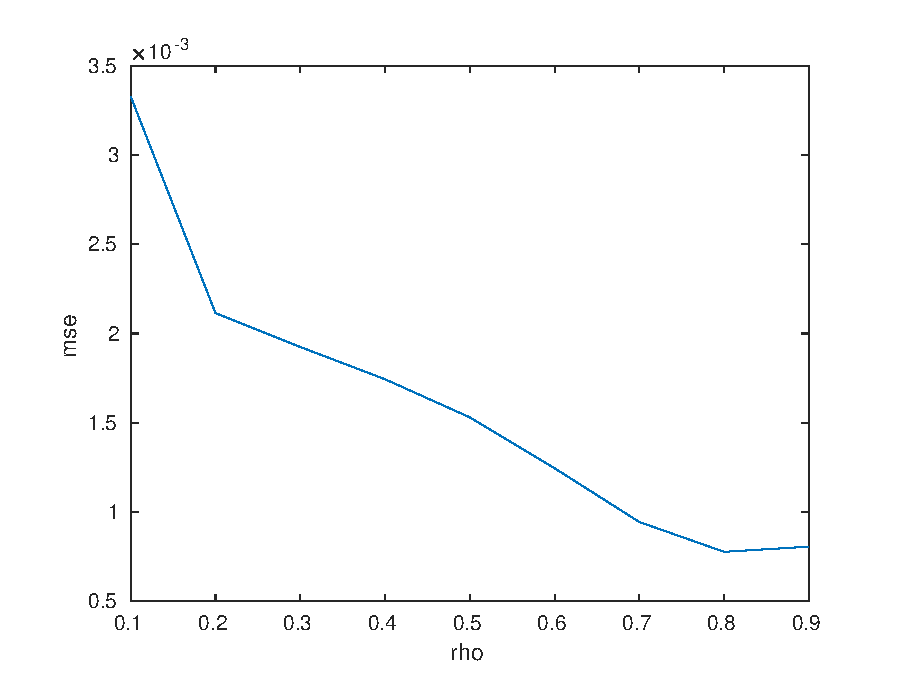
\includegraphics[width=0.7\linewidth]{immagini/trainingerror.eps}
	\caption{Training error generato da \textit{ESNtrain().}}
	\label{fig:trainingerror}
\end{figure}
L'errore di training è naturalmente più basso dell'errore di test che riflette comunque lo stesso andamento.\\
\begin{figure}[H]
	\centering 
	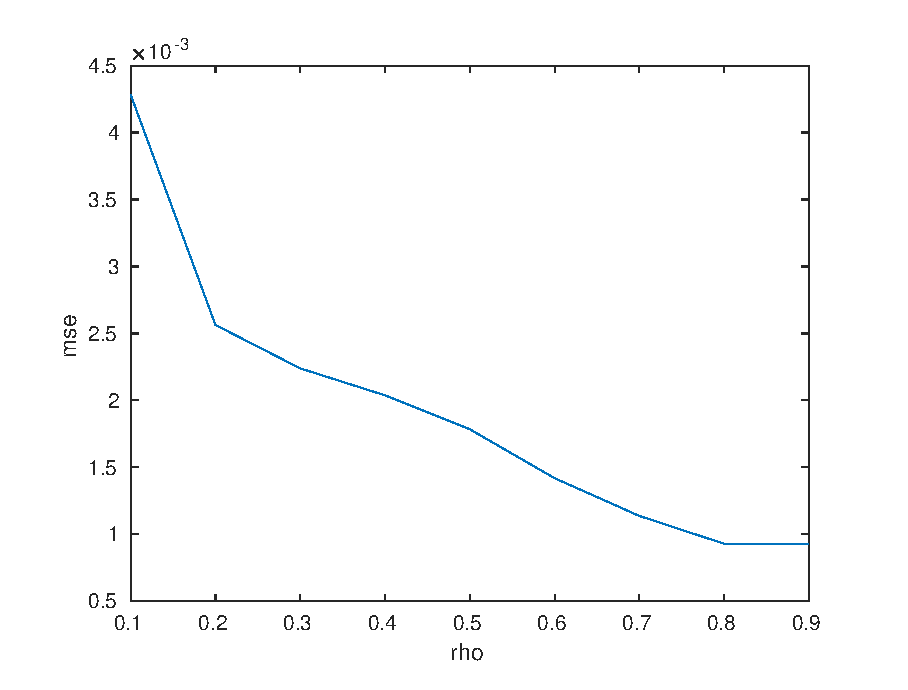
\includegraphics[width=0.6\linewidth]{immagini/testaftertrain}
	\caption{Test error generato da \textit{ESNtrain()} dopo l'allenameto del readout.}
	\label{fig:testaftertrain}
\end{figure}
\begin{figure}[H]
	\centering 
	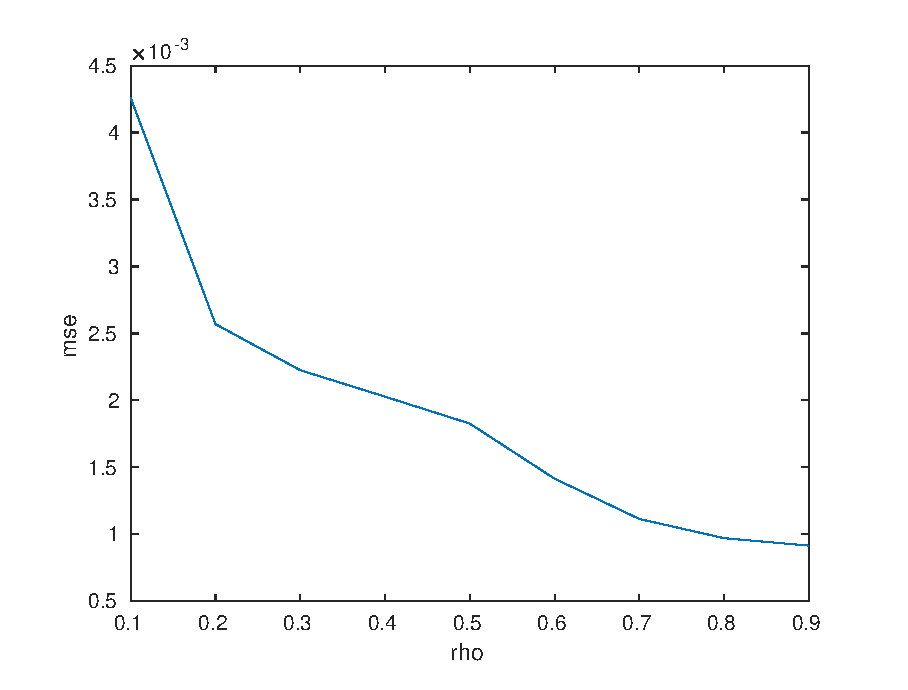
\includegraphics[width=0.6\linewidth]{immagini/testnewtrain}
	\caption{Test error generato da \textit{ESNtest()} dopo una nuova inizializzazione di \textit{reservoir}.}
	\label{fig:testnewtrain}
\end{figure}
\begin{figure}[H]
	\centering 
	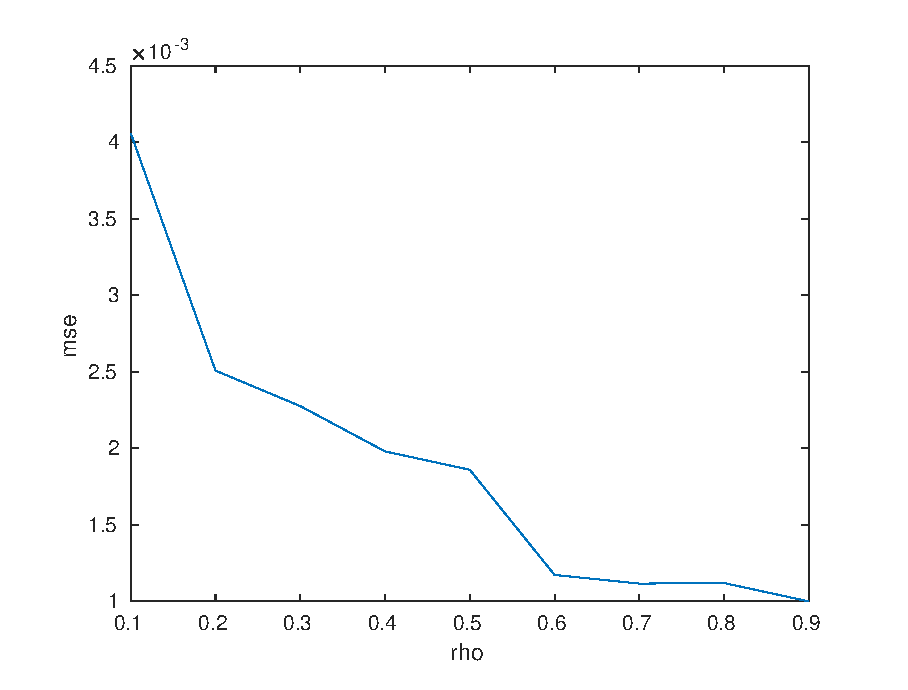
\includegraphics[width=0.6\linewidth]{immagini/testwout}
	\caption{Test error generato da \textit{ESNtest()} passando il readout già allenato.}
	\label{fig:testwout}
\end{figure}
Si può notare come l'errore diminuisca al crescere del valore del raggio spettrale, andamento aspettato nel caso di \textit{task} non lineare come questo.
Di seguito è mostrato il valore dell'\textit{input scaling} al variare del raggio spettrale. Nel paper questo valore è fissato prima della model selection proprio perchè imporre l'\textit{input scaling=0.1} risulta essere la scelta migliore.
\begin{figure}[H]
	\centering 
	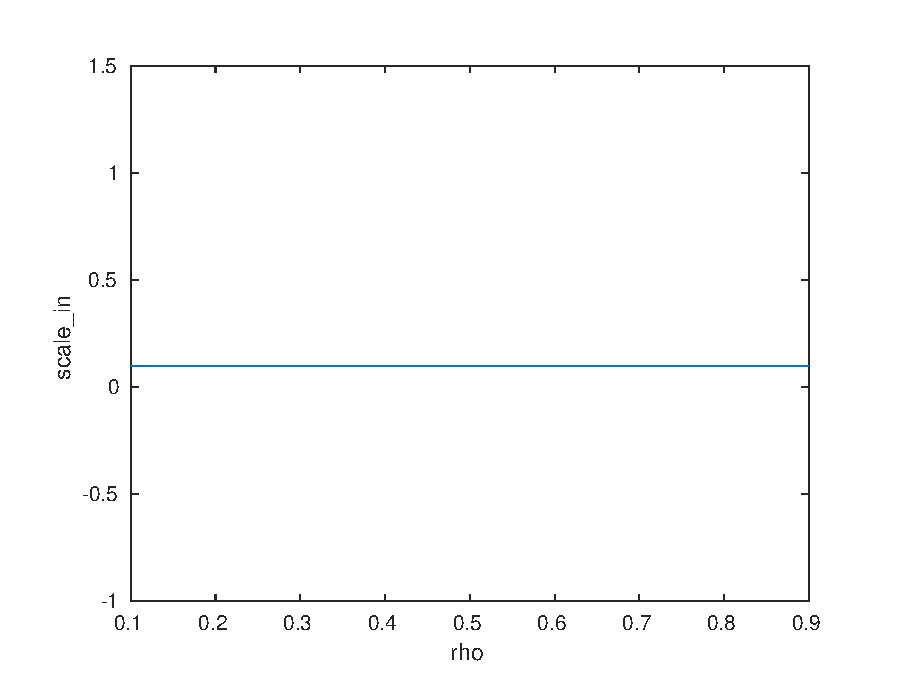
\includegraphics[width=0.6\linewidth]{immagini/scalein}
	\caption{Miglior scelta \textit{input scaling} al variare di rho.}
	\label{fig:scalein}
\end{figure}


Per avere un confronto preciso al livello numerico con il \textit{paper} citato, viene allenta una rete neurale con 500 unità totalmente connessa.
\begin{table}[h]
	\begin{center}
		\begin{tabular}{|c|c|}
			\hline
			Risultati paper & Risultati rete implementata \\
			\hline
			$3.1413 \times 10^{-4} (\pm1.14197 \times 10^{-5}) $ & 
			$3.2159 \times 10^{-4} (\pm1.1701 \times 10^{-5}) $\\
			\hline
		\end{tabular}
	\end{center}
\caption{Error test \textit{ESNtrain()}}
\end{table}

\section{Conclusioni}
I risultati ottenuti con la rete implementata dimostrano il corretto funzionamento di quest'ultima. La rete può dunque essere utilizzata per la computazione di altri \textit{task}, come quelli inseriti nella funzione per la generazione degli stessi. Il modello dunque risulta utile per un primo approccio alle \textit{Echo State Network} e come punto di partenza per la realizzazione di altri modelli. La sua modularità è stata pensata proprio per poter facilitare l'implementazione di reti con configurazioni diverse del \textit{reservoir} per studi futuri.


